%
% CHAPTER Versuch 1
%
\chapter{Bestimmung der Tonhöhe eines akustischen Signals}
\label{chap:VERSUCH_1}
Bestimmen der Frequenz eines Tones und Anwendung der Fouriertransformation.
 
\section{Fragestellung, Messprinzip, Aufbau, Messmittel}
\label{chap:VERSUCH_1_FRAGESTELLUNG}
In diesem ersten Versuch soll die Tonhöhe eines akustischen Signals bestimmt werden. Als akustischer Signalgeber wird eine Mundharmonika verwendet. Bei jener werden Töne durch einzelne dicht aneinander liegende Luftkanäle erzeugt.Deshalb ist es für einen Laien nicht auf Anhieb möglich einen Ton einzelnen zu spielen. Damit für den Versuch genau ein Ton zu hören ist, werden alle Luftkanäle bis auf einen mit Klebeband verschlossen.
Der Ton der Mundharmonika wird mit einem Mikrophon aufgenommen, welches an einem Oszilloskop angeschlossen ist. 
Da die Signale in analoger Form vorliegen, muss für die weitere Verarbeitung des Signals eine Digitalisierung vorgenommen werden.
Dabei ist das Abtastintervall $\Delta t$ gerade der zeitliche Abstand zwischen zwei Messungen. Die Abtastfrequenz ist gerade der Kehrwert zum Abtastintervall $\frac{1}{\Delta t}$. Diese Werte können im Unterabschnitt Messwerte in der Tabelle \ref{tab:Eigenschaften} entnommen werden. Die Digitalisierung erfolgt durch das Oszilloskop.
\\
Um einen Signalausschnitt aufzunehmen wird der "\textit{Single Sequence}" Modus im Oszilloskop eingestellt. Mit einem Pythonskript wird anschließend 2500 Messwerte vom Oszilloskop ausgelesen.
Aus diesem Signal im Zeitbereich wird das Spektrum mit Hilfe der Fouriertransformation berechnet. Die Umrechnung in das Amplitudenspektrum erfolgt mit Hilfe der Numpy Funktion $np.fft.fft()$, die auf der X-Achse jedoch nicht die Frequenz aufträgt, sondern die Einheit \textit{Anzahl Schwingungen innerhalb der gesamten Signaldauer}. Interessant ist jedoch die Frequenz. Deshalb muss diese noch mit folgender Formel errechnet werden.
\begin{equation}
f = \dfrac{n}{M \cdot \Delta t}
\end{equation}




\section{Messwerte}
\label{chap:VERSUCH_1_MESSWERTE}


\begin{table}[H]
\centering
\begin{tabular}{l|r}
Eigenschaft & Wert \\ \hline
Grundfrequenz in Hz & 917.43\\
Grundperiode in ms & 1.09\\
Abtastfreq in kHz & 100\\
Signaldauer in s & 0.025\\
Abtastinterval $\Delta t$ in s & $1 \cdot 10^{-5}s$\\
Signalänge $M$ Abtastungen & 2500\\
\end{tabular}
\caption{Eigenschaften der Messung und Grundfrequenz des Tones}
\label{tab:Eigenschaften}
\end{table}

\begin{figure}[H]
\centering
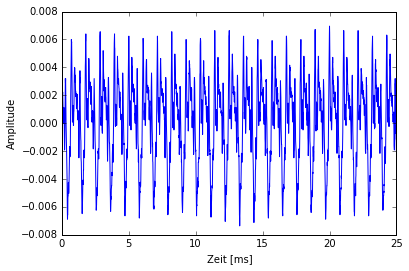
\includegraphics[width=170mm]{tone.png}
\caption{Signal im Zeitbereich}
\label{img:SIGNALZEITBEREICH}
\end{figure}

\begin{figure}[H]
\centering
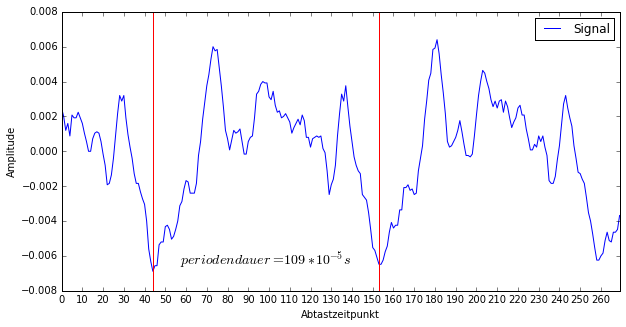
\includegraphics[width=165mm]{periodendauer.png}
\caption{Ausschnitt Signal im Zeitbereich mit eingezeichneter Periode}
\label{img:SIGNALPERIODE}
\end{figure}


\begin{figure}[H]
\centering
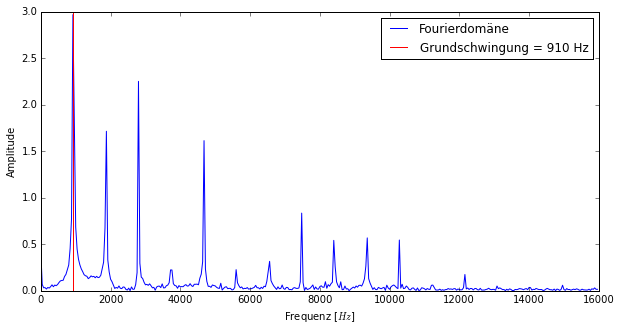
\includegraphics[width=165mm]{fft.png}
\caption{Signal in der Fourierdomäne}
\label{img:FFT}
\end{figure}

\section{Auswertung und Interpretation}
\label{chap:VERSUCH_1_AUSWERTUNG}
In Bild \ref{img:SIGNALZEITBEREICH} ist das Signal der Mundharmonika im Zeitbereich zu sehen. Auf den ersten Blick scheint es sich wie erwartet um ein periodisches Signal zu handeln. Auf der X-Achse ist die Zeit in Millisekunden und auf der Y-Achse die Amplitude in Volt aufgetragen. Nun soll die Grundfrequenz, sowie die Grundperiodendauer aus dem Signal im Zeitbereich bestimmt werden. Dafür wird ein vergrößerter Signalausschnitt unter die Lupe genommen. Dieser Bereich ist in Bild \ref{img:SIGNALPERIODE} zu sehen. 
Diesmal sind auf der X-Achse jedoch die einzelnen Abtastzeitpunkte aufgetragen. Die Y-Achse bleibt wie gehabt die Amplitude. Eine Periode beginnt mit einem "absolutem" Minima und endet mit einem "absolutem" Minima. Die Zeit die dazwischen vergeht ist die Periodendauer. Um an diese Zeit zu kommen wird das Abtastintervall $\Delta t$ und die Anzahl an Abtastungen benötigt. Die Periodendauer ergibt sich aus der Formel $T = n \cdot \Delta t$, wobei $T$ die Periodendauer, $n$ die Anzahl an Abtastungen und $\Delta t$ das Abtastintervall ist. Die korrespondierende Frequenz ist auf die übliche Weise zu berechnen. Die Grundfrequenz und die Grundperiode können in Tabelle \ref{tab:Eigenschaften} abgelesen werden. Die Grundfrequenz von 917.43 Hz liegt zwischen den Frequenzen der Töne a'' und b''. Es handelt sich bei dem Signal nicht um einen Reinen Sinuston, was man an dem Ausschnitt aus Bild \ref{img:SIGNALPERIODE} erkennen kann. 
Es handelt sich um eine Mischung verschiedener Frequenzen, welche ganzzahlige Vielfache der Grundfrequenz sind. Dies sind die sogenannten Obertöne, welche gerade die Melodie einer Mundharmonika ausmachen. So unterscheiden sich Instrumente, die den selben Ton spielen bei exakter Stimmung nicht in Ihrer Grundfrequenz, sondern lediglich im Bereich der höheren Harmonischen. Diese Obertöne können am besten in der Fourierdomäne erkannt werden. 
Das Spektrum des Signals ist in Bild \ref{img:FFT} zu sehen. Der erste Peak im Spektrum ist die Grundfrequenz. Alle weiteren Peaks sollten ganzzahlige Vielfache dieser sein, gut erkennbar sind $1 bis 10 und 12$, zu beachten ist, dass das in der Grafik gezeigte Diagramm bei 16000 Hz endet, die Funktion $fft.fft()$ liefert noch deutlich mehr werte, welche allerdings keine Peaks mehr enthalten und somit für uns uninteressant sind. Aus dem Spektrum kann die Grundfrequenz mit 910 Hz bestimmt werden $(rote Linie in der Grafik)$. Die aus dem Zeitbereich abgelesene Grundfrequenz unterscheidet sich zu der im Amplitudenspektrum abgelesenen um $\approx 1\%$.
